\documentclass[a4paper]{article}

% Because it looks better:
\usepackage{a4wide}
% Take care of input things:
\usepackage[utf8]{inputenc}
\usepackage[T1]{fontenc}
% Packages for pictures:
\usepackage{graphicx}
\usepackage{float}
\usepackage{listings}
\lstset{numbers=left, numberstyle=\tiny, numbersep=5pt
,frame=single, captionpos=b}
\lstset{language=Perl}
% Package for urls:
\usepackage{url}

%\bibliographystyle{alpha}

% Now let us define a few shortcuts:
% Correct sign for C#:
\newcommand{\CS}{C\nolinebreak\hspace{-.05em}\raisebox{.6ex}{\scriptsize\bf \#\ }}

% --------------------------------------------------------------------------------------------!
%
% NOTE: For better usage of LaTeX with GIT, please write each sentence on an own line, separating paragraphs
%       by the usual double returns. That way GIT can track each sentence on its own instead of always
%       having to track a paragraph as one block.
%
% --------------------------------------------------------------------------------------------!

\begin{document}

\title{Documentation}
\author{Andreas Köll, Johannes Bohner, Burkhard Hoppenstedt, Tamino Hartmann}
\date{\today}

\maketitle

\begin{abstract}

Abstract here
\end{abstract}
\newpage

\section{Introduction}

This paper represents a rework of \cite{origin}.
We analyzed what the authors did and tried the method on a somewhat different study.
Here we show the documentation to our work, our conclusions, and how our work compares to the original work.

\section{Overview of Decomposing Biological Motion}

This section will briefly highlight interesting and important aspects from the original paper on which our work was based on.
The general goal of the paper was to implement a system on the computer capable of interpreting biological motion.
This was done by recording the walking motion of men and women with a motion capturing system on a treadmill and then putting the data through an algorithm to distinguish between the gender based on the biological motion.

As the recorded data was not insignificant in its size, a principle component analysis was used to decrease the data volume.
The original authors found that the first four principal components offered sufficient coverage of the data with a value of 98\%.\footnote{TODO: Sollen wir hier auch noch die Grafik einfügen? Eigentlich unnötig...}
Just the standard poses and their principal components however do not represent movement: they must be animated over time.
This was done by mapping the values to a sinus function modified by its parameters.\footnote{TODO: Evtl. die Parameter aufzählen? Brauchen wir das?}
The data could then be represented in a single, 229 dimensional vector consisting of the three components: the standard poses, the principal components, and the parameters for the sinus function.

The data from all the walkers was then analyzed by a simple linear comparison algorithm.
The computer managed to correctly classify 90\% correctly in the best case (dependent on the various different approaches).
This was better than the control group's average.

Finally, the authors used the algorithm backwards to synthesize stylized walkers.
These can be changed interactively, allowing a quick comparison between the two distinct extremes between the genders and any step between.

\section{REWORK: Setup of the Experiment}

This section describes the way the data was recorded to the best of our abilities.
We'll first look at the hardware and software side of things and then continue on to the actual proceedings that were established to capture the motion data required for the analysis.

\subsection{REWORK: Equipment}

For our recording we used the "Kinect for Windows"\texttrademark \cite{kinect}, connected to a computer running "Microsoft Windows 7"\textregistered \ via USB.
The Kinect is mounted on a tripod to allow correct positioning.
The weights were applied with a weight-vest with a weight of 5 kilograms.
For the alternate motion, skipping, we also provided a rope.
We used normal tape to mark positions on the floor so that all recordings were made with the same measurements.

\subsection{REWORK: Software}

We developed our own application for recording the input stream from the Kinect in \CS with "Microsoft Visual Studio 2012" utilizing the "Microsoft Kinect Developer Version".
The program is currently available as open source here \cite{csprogram} and can be seen in Fig ~\ref{fig:programm}.

\begin{figure}[H]
	\centering
	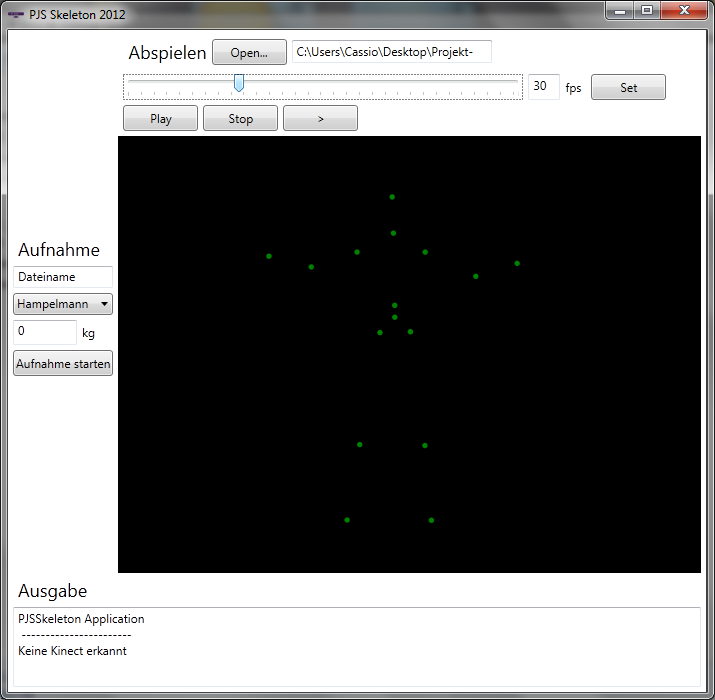
\includegraphics[width=8cm]{programm.jpg}
	\caption{Screenshot of the program used to record the data.}
	\label{fig:programm}
\end{figure}

Later steps that were based on the recorded data were programmed in MATLAB, available here \cite{matlabprograms}.

\subsection{REWORK: Workflow}

As the overall workflow of the data from its capture to final results is non-trivial, we have provided a flowchart of the procedure to help understand what code does what when and which data files represent what intermediate results\footnote{TODO: Add flowchart here!}.

\subsection{REWORK: Composition of the Recording}

Figure \ref{fig:schematic} shows the schematics of the arrangement of the Kinect for the recordings\footnote{TODO: Change figure to have english text!}.
The way the Kinect records skeletons proved to be a strong limiting factor in selecting which motions to record as the depth-perception is comparatively poor.
The fixed nature of the experiment also limited the motion to one that could be done within a small area, which disclosed for example any form of walking or running.

\begin{figure}
	\centering
	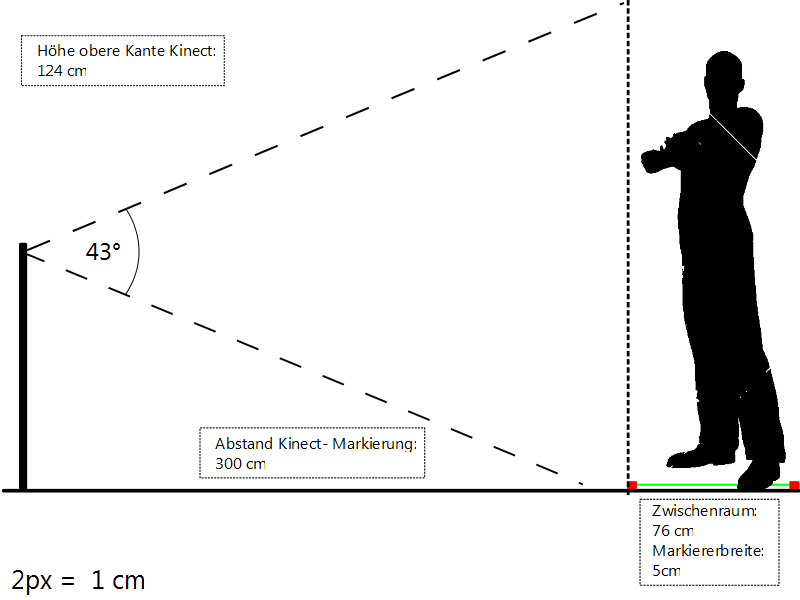
\includegraphics[width=10cm]{Aufbau.png}
	\caption{Schematics of the arrangement for the recording of our source data.}
	\label{fig:schematic}
\end{figure}

\section{Creating Motionvectors to Represent Motion Data}

Having saved all of the skeleton data received from the Kinect into textfields the representation of the jumping motion of every subject is a huge matrix. Each row of this matrix represents one single posture of the subject's body, which consists of 48 values: Each of the 16 joints is represented by three floating-point numbers specifying the three-dimensional position of the joint.

This data is highly redundant. For example, jumping jack and jump rope are symmetrical motions. The right arm moves the same way as the left arm does except for reflection. The same goes for the legs.

\section{Visualisation}

This section is independent from the rest of the paper as the analytical methods don't matter. Out intent is to show the captured points of the skeleton in an representative 3D Model.

\subsection{Absolute vs. Relative Values}
As seen in the description of storing points in a ".txt" file the kinect uses Absolute Values to represent the skeleton  - which is absolutely useful, because otherwise it couldn't detect different lengths in body parts. Instead it would had to map the measured values on a defined body model. This procedure would cause inaccuracy.\
While animating a defined model in the opposite you can't just easily scale single body parts to adjust the proportions. This problem needs as a solution a format invariant to scaling.

\subsection{The .bvh file}
The software used for testing the following part is Poser 9 from SmithMicro.\footnote{http://www.software3d.de/figurendesign/smithmicro-poser-9.html}
A .bvh file is made up of two parts: The bodystructure and the frames.\
The bodystructure defines the relationship between each bodypart. As one might see in
Listing 1 this structure is build hierarchical. Each joint is represented by a name and the connection to its successors. Changing the value in a joint affects all the successors. 
The standardpose (all angles in between 0) is the so called T-Pose. You can see the model standing with parallel feet looking straight forward and the arms are bend 90 degrees relative to the body.
\begin{lstlisting}[caption=.bvh Connected Structure]{Name}
JOINT lCollar
{
		OFFSET	1.858774 10.237258 -1.915852
		CHANNELS 3 Zrotation Yrotation Xrotation
		JOINT lShldr
		{
			OFFSET	6.103279 0.000102 -0.038601
			CHANNELS 3 Zrotation Yrotation Xrotation
			JOINT lForeArm
\end{lstlisting}

Responseable for the change over time is the second part of the file. In here we define the joint-angles. Really useful for this aspect of the project was the similarity between the recorded ".txt" file and the seond part of the ".bvh". Therefore we could calculate the absolute positions in a row from the .txt-File to angles and replace the current lines in the .bvh by the ones generated by a matlab script which will be shown in the following section.
\begin{lstlisting}[caption=Motionpart of .bvh]{Name}
MOTION
Frames:     160
Frame Time: 1                
0 50.946 0 0 0 0 0 0 0 0 0 0 0 0 0 0 -30.66 0 0 -30.295 0 0 10.811 ...
0 51.229 0 0 0 0 0 0 0 0 0 0 0 0 0 0 -29.93 0 0 -30.695 0 0 9.6152 ...
\end{lstlisting}

\subsection{Calculating the angles}
After finding the corresponding entries in the ".txt" and ".bvh" file now is the time to convert values. Using Matlab as  intermediary between the two formats we take the advantage of easy handling .txt to matrices.

\begin{lstlisting}[caption=Calculating the angle]{Name}
D = dlmread('nameSeilhuepfen0.txt');
[...]

# Rechter Oberarm Eintrag Nr.25 (Vektor 24x Daten sind schon vorhanden)
m46 = (D(ind,17)-D(ind,11))/(D(ind,16)-D(ind,10));

# Vektorenberechnung. Nummerierung erfolgt von Punktnummer 
# aus Kinectmodells
Vektor46y = D(ind,17)-D(ind,11);
Vektor46x = D(ind,16)-D(ind,10);
skalarprodukt=Vektor24y*Vektor46y+Vektor24x*Vektor46x;
laengeeins=sqrt(Vektor24y^2 + Vektor24x^2);
laengezwei=sqrt(Vektor46y^2 + Vektor46x^2); 
wOberarm_rechts = radtodeg(acos(skalarprodukt/(laengeeins*laengezwei)));
\end{lstlisting}

\section{Conclusion}

TODO: Put conclusion here.

\newpage
\bibliography{doc.bib}

\end{document}